% questions.tex —— 2017 年·全国Ⅱ卷·理科 · 题目内容片段（无答案）
% 由 tools/generate_projects.py 依来源总账自 2017/2017_数学真题_全国2理_试题.md 生成，勿手改（改源 MD 后重跑）


\gkpart{数学}

\begin{gktip}
\textbf{来源说明}：本题面依据固定源 PDF 两页 A3 页面逐题核对，原卷印刷页码 1041–1042。固定源不附答案；本文件仅为题面规范源。
\end{gktip}

\gkpart{一、选择题}

\begin{question}
\gkti{1}\(\dfrac{3+i}{1+i}=\)（　）

   (A) \(1+2i\)　　(B) \(1-2i\)　　(C) \(2+i\)　　(D) \(2-i\)

\end{question}
\begin{question}
\gkti{2}设集合 \(A=\{1,2,4\}\)，\(B=\{x\mid x^2-4x+m=0\}\)。若 \(A\cap B=\{1\}\)，则 \(B=\)（　）

   (A) \(\{1,-3\}\)　　(B) \(\{1,0\}\)　　(C) \(\{1,3\}\)　　(D) \(\{1,5\}\)

\end{question}
\begin{question}
\gkti{3}我国古代数学名著《算法统宗》中有如下问题：“远望巍巍塔七层，红光点点倍加增，共灯三百八十一，请问尖头几盏灯？”意思是：一座 7 层塔共挂了 381 盏灯，且相邻两层中的下一层灯数是上一层灯数的 2 倍，则塔的顶层共有灯（　）

   (A) 1 盏　　(B) 3 盏　　(C) 5 盏　　(D) 9 盏

\Needspace{0.4\textheight}
\end{question}
\begin{question}
\gkti{4}如图，网格纸上小正方形的边长为 1，粗实线画出的是某几何体的三视图，该几何体由一平面将一圆柱截去一部分后所得，则该几何体的体积为（　）
\nopagebreak[4]
\begin{center}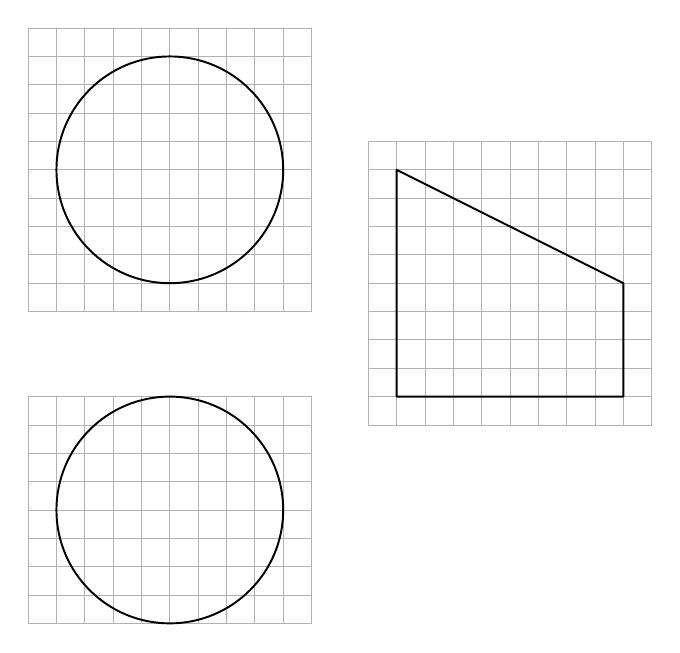
\begin{tikzpicture}[line cap=round,line join=round,line width=0.7pt,scale=0.36]
\begin{scope}[shift={(0,11)}]
  \draw[gray!60,line width=0.3pt] (0,0) grid (10,10);
  \draw (5,5) circle (4);
\end{scope}
\begin{scope}[shift={(12,7)}]
  \draw[gray!60,line width=0.3pt] (0,0) grid (10,10);
  \draw (1,1)--(9,1)--(9,5)--(1,9)--cycle;
\end{scope}
\begin{scope}
  \draw[gray!60,line width=0.3pt] (0,0) grid (10,8);
  \draw (5,4) circle (4);
\end{scope}
\end{tikzpicture}
\end{center}
\nopagebreak[4]
   (A) \(90\pi\)　　(B) \(63\pi\)　　(C) \(42\pi\)　　(D) \(36\pi\)

\end{question}
\begin{question}
\gkti{5}设 \(x,y\) 满足约束条件
\nopagebreak[4]
\[
   \begin{cases}
   2x+3y-3\leq 0,\\
   2x-3y+3\geq 0,\\
   y+3\geq 0,
   \end{cases}
\]
   则 \(z=2x+y\) 的最小值是（　）

   (A) \(-15\)　　(B) \(-9\)　　(C) \(1\)　　(D) \(9\)

\end{question}
\begin{question}
\gkti{6}安排 3 名志愿者完成 4 项工作，每人至少完成 1 项，每项工作由 1 人完成，则不同的安排方式共有（　）

   (A) 12 种　　(B) 18 种　　(C) 24 种　　(D) 36 种

\end{question}
\begin{question}
\gkti{7}甲、乙、丙、丁四位同学一起去向老师询问成语竞赛的成绩。老师说：你们四人中有 2 位优秀，2 位良好，我现在给甲看乙、丙的成绩，给乙看丙的成绩，给丁看甲的成绩。看后甲对大家说：我还是不知道我的成绩。根据以上信息，则（　）

   (A) 乙可以知道四人的成绩　　(B) 丁可以知道四人的成绩

   (C) 乙、丁可以知道对方的成绩　　(D) 乙、丁可以知道自己的成绩

\Needspace{0.4\textheight}
\end{question}
\begin{question}
\gkti{8}执行如图的程序框图，如果输入的 \(a=-1\)，则输出的 \(S=\)（　）
\nopagebreak[4]
\begin{center}\begin{tikzpicture}[line width=0.75pt,line cap=round,line join=round,font=\small]
\node[draw,rounded corners,minimum width=1.35cm,minimum height=0.5cm] (start) at (0,0) {开始};
\node[draw,minimum width=2.2cm,minimum height=0.55cm] (input) at (0,-0.95) {输入 $a$};
\node[draw,minimum width=2.7cm,minimum height=0.55cm] (init) at (0,-1.9) {$S=0,\ K=1$};
\coordinate (dt) at (0,-2.6);
\coordinate (dr) at (1.9,-3.2);
\coordinate (db) at (0,-3.8);
\coordinate (dl) at (-1.9,-3.2);
\draw (dt)--(dr)--(db)--(dl)--cycle;
\node at (0,-3.2) {$K\le 6$};
\node[draw,minimum width=3.0cm,minimum height=0.55cm] (sum) at (0,-4.55) {$S=S+a\cdot K$};
\node[draw,minimum width=2.3cm,minimum height=0.55cm] (flip) at (0,-5.45) {$a=-a$};
\node[draw,minimum width=2.6cm,minimum height=0.55cm] (next) at (0,-6.35) {$K=K+1$};
\node[draw,minimum width=1.9cm,minimum height=0.55cm] (out) at (3.6,-3.2) {输出 $S$};
\node[draw,rounded corners,minimum width=1.35cm,minimum height=0.5cm] (end) at (3.6,-4.2) {结束};
\draw[->] (start)--(input);
\draw[->] (input)--(init);
\draw[->] (init)--(dt);
\draw[->] (db)--node[right]{是}(sum);
\draw[->] (sum)--(flip);
\draw[->] (flip)--(next);
\draw[->] (next.west)--(-2.65,-6.35)--(-2.65,-3.2)--(dl);
\draw[->] (dr)--node[above]{否}(out.west);
\draw[->] (out)--(end);
\end{tikzpicture}
\end{center}
\nopagebreak[4]
   (A) 2　　(B) 3　　(C) 4　　(D) 5

\end{question}
\begin{question}
\gkti{9}若双曲线 \(C:\dfrac{x^2}{a^2}-\dfrac{y^2}{b^2}=1\)（\(a>0,b>0\)）的一条渐近线被圆 \((x-2)^2+y^2=4\) 所截得的弦长为 2，则 \(C\) 的离心率为（　）

   (A) \(2\)　　(B) \(\sqrt{3}\)　　(C) \(\sqrt{2}\)　　(D) \(\dfrac{2\sqrt{3}}{3}\)

\end{question}
\begin{question}
\gkti{10}已知直三棱柱 \(ABC-A_1B_1C_1\) 中，\(\angle ABC=120^\circ\)，\(AB=2\)，\(BC=CC_1=1\)，则异面直线 \(AB_1\) 与 \(BC_1\) 所成角的余弦值为（　）

   (A) \(\dfrac{\sqrt{3}}{2}\)　　(B) \(\dfrac{\sqrt{15}}{5}\)　　(C) \(\dfrac{\sqrt{10}}{5}\)　　(D) \(\dfrac{\sqrt{3}}{3}\)

\end{question}
\begin{question}
\gkti{11}若 \(x=-2\) 是函数 \(f(x)=(x^2+ax-1)e^{x-1}\) 的极值点，则 \(f(x)\) 的极小值为（　）

   (A) \(-1\)　　(B) \(-2e^{-3}\)　　(C) \(5e^{-3}\)　　(D) \(1\)

\end{question}
\begin{question}
\gkti{12}已知 \(\triangle ABC\) 是边长为 2 的等边三角形，\(P\) 为平面 \(ABC\) 内一点，则 \(\overrightarrow{PA}\cdot(\overrightarrow{PB}+\overrightarrow{PC})\) 的最小值是（　）

   (A) \(-2\)　　(B) \(-\dfrac{3}{2}\)　　(C) \(-\dfrac{4}{3}\)　　(D) \(-1\)

\end{question}
\gkpart{二、填空题}

\begin{question}
\gkti{13}一批产品的二等品率为 0.02，从这批产品中每次随机取一件，有放回地抽取 100 次，\(X\) 表示抽到的二等品件数，则 \(DX=\)\gkblank{}。

\end{question}
\begin{question}
\gkti{14}函数 \(f(x)=\sin^2x+\sqrt{3}\cos x-\dfrac{3}{4}\)（\(x\in[0,\dfrac{\pi}{2})\)）的最大值是\gkblank{}。

\end{question}
\begin{question}
\gkti{15}等差数列 \(\{a_n\}\) 的前 \(n\) 项和为 \(S_n\)，\(a_3=3\)，\(S_4=10\)，则 \(\displaystyle\sum_{k=1}^{n}\dfrac{1}{S_k}=\)\gkblank{}。

\end{question}
\begin{question}
\gkti{16}已知 \(F\) 是抛物线 \(C:y^2=8x\) 的焦点，\(M\) 是 \(C\) 上一点，\(FM\) 的延长线交 \(y\) 轴于点 \(N\)。若 \(M\) 为 \(FN\) 的中点，则 \(|FN|=\)\gkblank{}。

\end{question}
\gkpart{三、解答题}

\begin{question}
\gkti{17}\(\triangle ABC\) 的内角 \(A,B,C\) 的对边分别为 \(a,b,c\)，已知 \(\sin(A+C)=8\sin^2\dfrac{B}{2}\)。

   (1) 求 \(\cos B\)；

   (2) 若 \(a+c=6\)，\(\triangle ABC\) 面积为 2，求 \(b\)。

\Needspace{0.4\textheight}
\end{question}
\begin{question}
\gkti{18}海水养殖场进行某水产品的新、旧网箱养殖方法的产量对比，收获时各随机抽取了 100 个网箱，测量各箱水产品的产量（单位：kg），其频率分布直方图如图：
\nopagebreak[4]
\begin{center}\begin{tikzpicture}[x=0.68cm,y=0.68cm,line width=0.55pt,font=\scriptsize]
\begin{scope}
  \draw[->] (0,0)--(9.45,0);
  \draw[->] (0,0)--(0,7.55);
  \foreach \y/\lab/\x in {1.2/0.012/0,1.4/0.014/-1,2.0/0.020/0,2.4/0.024/0,3.2/0.032/0,3.4/0.034/-1,4.0/0.040/0} {
    \draw[densely dashed,gray] (0,\y)--(9,\y);
    \node[left] at (\x,\y) {\lab};
  }
  \foreach \x/\lab in {0/25,1/30,2/35,3/40,4/45,5/50,6/55,7/60,8/65,9/70} {
    \draw (\x,0)--(\x,-0.08);
    \node[below] at (\x,-0.12) {\lab};
  }
  \foreach \x/\h in {0/1.2,1/1.4,2/2.4,3/3.4,4/4.0,5/3.2,6/2.0,7/1.2,8/1.2} {
    \draw[fill=white] (\x,0) rectangle ++(1,\h);
  }
  \node[anchor=west] at (0.18,7.15) {频率/组距};
  \node at (4.5,-0.9) {箱产量/kg};
  \node at (4.5,-1.55) {旧养殖法};
\end{scope}
\begin{scope}[shift={(12,0)}]
  \draw[->] (0,0)--(7.45,0);
  \draw[->] (0,0)--(0,7.55);
  \foreach \y/\lab/\x in {0.4/0.004/0,0.8/0.008/-1,1.0/0.010/0,2.0/0.020/0,4.4/0.044/0,4.6/0.046/-1,6.8/0.068/0} {
    \draw[densely dashed,gray] (0,\y)--(7,\y);
    \node[left] at (\x,\y) {\lab};
  }
  \foreach \x/\lab in {0/35,1/40,2/45,3/50,4/55,5/60,6/65,7/70} {
    \draw (\x,0)--(\x,-0.08);
    \node[below] at (\x,-0.12) {\lab};
  }
  \foreach \x/\h in {0/0.4,1/2.0,2/4.4,3/6.8,4/4.6,5/1.0,6/0.8} {
    \draw[fill=white] (\x,0) rectangle ++(1,\h);
  }
  \node[anchor=west] at (0.18,7.15) {频率/组距};
  \node at (3.5,-0.9) {箱产量/kg};
  \node at (3.5,-1.55) {新养殖法};
\end{scope}
\end{tikzpicture}
\end{center}
\nopagebreak[4]
   (1) 设两种养殖方法的箱产量相互独立，记 \(A\) 表示事件“旧养殖法的箱产量低于 50 kg，新养殖法的箱产量不低于 50 kg”，估计 \(A\) 的概率；

   (2) 填写下面列联表，并根据列联表判断是否有 99\% 的把握认为箱产量与养殖方法有关；

\begin{center}
\begin{tabular}{lrr}
\toprule
 & 箱产量 < 50 kg & 箱产量 $\geq$ 50 kg \\
\midrule
旧养殖法 &  &  \\
新养殖法 &  &  \\
\bottomrule
\end{tabular}
\end{center}

   (3) 根据箱产量的频率分布直方图，求新养殖法箱产量的中位数的估计值（精确到 0.01）。

\Needspace{10\baselineskip}
   附：

\begin{center}
\begin{tabular}{lrrr}
\toprule
\(P(K^2\geq k)\) & 0.050 & 0.010 & 0.001 \\
\midrule
\(K\) & 3.841 & 6.635 & 10.828 \\
\bottomrule
\end{tabular}
\end{center}

\nopagebreak[4]
\[
   K^2=\frac{n(ad-bc)^2}{(a+b)(c+d)(a+c)(b+d)}.
\]

\Needspace{0.4\textheight}
\end{question}
\begin{question}
\gkti{19}如图，在四棱锥 \(P-ABCD\) 中，侧面 \(PAD\) 为等边三角形且垂直于底面 \(ABCD\)，\(AB=BC=\dfrac{1}{2}AD\)，\(\angle BAD=\angle ABC=90^\circ\)，\(E\) 是 \(PD\) 的中点。
\nopagebreak[4]
\begin{center}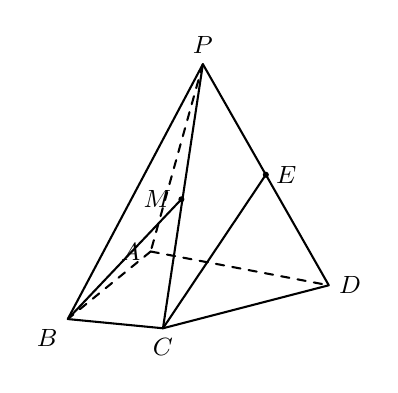
\begin{tikzpicture}[x=0.78cm,y=0.78cm,line cap=round,line join=round,line width=0.75pt,font=\small]
\coordinate (A) at (1.35,1.1);
\coordinate (B) at (0,0);
\coordinate (C) at (1.55,-0.15);
\coordinate (D) at (4.25,0.55);
\coordinate (P) at (2.2,4.15);
\coordinate (M) at (1.85,1.95);
\coordinate (E) at (3.225,2.35);
\draw (P)--(B)--(C)--(D)--(P);
\draw (P)--(C);
\draw[dashed] (P)--(A);
\draw[dashed] (A)--(B);
\draw[dashed] (A)--(D);
\draw (B)--(M);
\draw (C)--(E);
\fill (M) circle (1.1pt);
\fill (E) circle (1.1pt);
\node[above] at (P) {$P$};
\node[below left] at (B) {$B$};
\node[below] at (C) {$C$};
\node[right] at (D) {$D$};
\node[left] at (A) {$A$};
\node[left] at (M) {$M$};
\node[right] at (E) {$E$};
\end{tikzpicture}
\end{center}
\nopagebreak[4]
   (1) 证明：直线 \(CE\parallel\) 平面 \(PAB\)；

   (2) 点 \(M\) 在棱 \(PC\) 上，且直线 \(BM\) 与底面 \(ABCD\) 所成角为 \(45^\circ\)，求二面角 \(M-AB-D\) 的余弦值。

\end{question}
\begin{question}
\gkti{20}设 \(O\) 为坐标原点，动点 \(M\) 在椭圆 \(C:\dfrac{x^2}{2}+y^2=1\) 上，过 \(M\) 作 \(x\) 轴的垂线，垂足为 \(N\)，点 \(P\) 满足 \(\overrightarrow{NP}=\sqrt{2}\,\overrightarrow{NM}\)。

   (1) 求点 \(P\) 的轨迹方程；

   (2) 设点 \(Q\) 在直线 \(x=-3\) 上，且 \(\overrightarrow{OP}\cdot\overrightarrow{PQ}=1\)。证明：过点 \(P\) 且垂直于 \(OQ\) 的直线 \(l\) 过 \(C\) 的左焦点 \(F\)。

\end{question}
\begin{question}
\gkti{21}已知函数 \(f(x)=ax^2-ax-x\ln x\)，且 \(f(x)\geq 0\)。

   (1) 求 \(a\)；

   (2) 证明：\(f(x)\) 存在唯一的极大值点 \(x_0\)，且 \(e^{-2}<f(x_0)<2^{-2}\)。

\end{question}
\begin{question}
\gkti{22}在直角坐标系 \(xOy\) 中，以坐标原点为极点，\(x\) 轴的正半轴为极轴建立极坐标系，曲线 \(C_1\) 的极坐标方程为 \(\rho\cos\theta=4\)。

   (1) \(M\) 为曲线 \(C_1\) 上的动点，点 \(P\) 在线段 \(OM\) 上，且满足 \(|OM|\cdot|OP|=16\)，求点 \(P\) 的轨迹 \(C_2\) 的直角坐标方程；

   (2) 设点 \(A\) 的极坐标为 \((2,\dfrac{\pi}{3})\)，点 \(B\) 在曲线 \(C_2\) 上，求 \(\triangle OAB\) 面积的最大值。

\end{question}
\begin{question}
\gkti{23}已知 \(a>0,b>0,a^3+b^3=2\)，证明：

   (1) \((a+b)(a^5+b^5)\geq 4\)；

   (2) \(a+b\leq 2\)。

\end{question}